\documentclass{article}
\usepackage[margin=1in]{geometry}
\usepackage[linesnumbered,ruled,vlined]{algorithm2e}
\usepackage{amsfonts}
\usepackage{amsmath}
\usepackage{amssymb}
\usepackage{amsthm}
\usepackage{enumitem}
\usepackage{fancyhdr}
\usepackage{hyperref}
\usepackage{minted}
\usepackage{multicol}
\usepackage{pdfpages}
\usepackage{standalone}
\usepackage[many]{tcolorbox}
\usepackage{tikz-cd}
\usepackage{transparent}
\usepackage{xcolor}
% \tcbuselibrary{minted}

\author{Nathan Solomon}

\newcommand{\fig}[1]{
    \begin{center}
        \includegraphics[width=\textwidth]{#1}
    \end{center}
}

% Math commands
\renewcommand{\d}{\mathrm{d}}
\DeclareMathOperator{\id}{id}
\DeclareMathOperator{\im}{im}
\DeclareMathOperator{\proj}{proj}
\DeclareMathOperator{\Span}{span}
\DeclareMathOperator{\Tr}{Tr}
\DeclareMathOperator{\tr}{tr}
\DeclareMathOperator{\ad}{ad}
\DeclareMathOperator{\ord}{ord}
%%%%%%%%%%%%%%% \DeclareMathOperator{\sgn}{sgn}
\DeclareMathOperator{\Aut}{Aut}
\DeclareMathOperator{\Inn}{Inn}
\DeclareMathOperator{\Out}{Out}
\DeclareMathOperator{\stab}{stab}

\newcommand{\N}{\ensuremath{\mathbb{N}}}
\newcommand{\Z}{\ensuremath{\mathbb{Z}}}
\newcommand{\Q}{\ensuremath{\mathbb{Q}}}
\newcommand{\R}{\ensuremath{\mathbb{R}}}
\newcommand{\C}{\ensuremath{\mathbb{C}}}
\renewcommand{\H}{\ensuremath{\mathbb{H}}}
\newcommand{\F}{\ensuremath{\mathbb{F}}}

\newcommand{\E}{\ensuremath{\mathbb{E}}}
\renewcommand{\P}{\ensuremath{\mathbb{P}}}

\newcommand{\es}{\ensuremath{\varnothing}}
\newcommand{\inv}{\ensuremath{^{-1}}}
\newcommand{\eps}{\ensuremath{\varepsilon}}
\newcommand{\del}{\ensuremath{\partial}}
\renewcommand{\a}{\ensuremath{\alpha}}

\newcommand{\abs}[1]{\ensuremath{\left\lvert #1 \right\rvert}}
\newcommand{\norm}[1]{\ensuremath{\left\lVert #1\right\rVert}}
\newcommand{\mean}[1]{\ensuremath{\left\langle #1 \right\rangle}}
\newcommand{\floor}[1]{\ensuremath{\left\lfloor #1 \right\rfloor}}
\newcommand{\ceil}[1]{\ensuremath{\left\lceil #1 \right\rceil}}
\newcommand{\bra}[1]{\ensuremath{\left\langle #1 \right\rvert}}
\newcommand{\ket}[1]{\ensuremath{\left\lvert #1 \right\rangle}}
\newcommand{\braket}[2]{\ensuremath{\left.\left\langle #1\right\vert #2 \right\rangle}}

\newcommand{\catname}[1]{{\normalfont\textbf{#1}}}

\newcommand{\up}{\ensuremath{\uparrow}}
\newcommand{\down}{\ensuremath{\downarrow}}

% Custom environments
\newtheorem{thm}{Theorem}[section]

\definecolor{probBackgroundColor}{RGB}{250,240,240}
\definecolor{probAccentColor}{RGB}{140,40,0}
\newenvironment{prob}{
    \stepcounter{thm}
    \begin{tcolorbox}[
        boxrule=1pt,
        sharp corners,
        colback=probBackgroundColor,
        colframe=probAccentColor,
        borderline west={4pt}{0pt}{probAccentColor},
        breakable
    ]
    \color{probAccentColor}\textbf{Problem \thethm.} \color{black}
} {
    \end{tcolorbox}
}

\definecolor{exampleBackgroundColor}{RGB}{212,232,246}
\newenvironment{example}{
    \stepcounter{thm}
    \begin{tcolorbox}[
      boxrule=1pt,
      sharp corners,
      colback=exampleBackgroundColor,
      breakable
    ]
    \textbf{Example \thethm.}
} {
    \end{tcolorbox}
}

\definecolor{propBackgroundColor}{RGB}{255,245,220}
\definecolor{propAccentColor}{RGB}{150,100,0}
\newenvironment{prop}{
    \stepcounter{thm}
    \begin{tcolorbox}[
        boxrule=1pt,
        sharp corners,
        colback=propBackgroundColor,
        colframe=propAccentColor,
        breakable
    ]
    \color{propAccentColor}\textbf{Proposition \thethm. }\color{black}
} {
    \end{tcolorbox}
}

\definecolor{thmBackgroundColor}{RGB}{235,225,245}
\definecolor{thmAccentColor}{RGB}{50,0,100}
\renewenvironment{thm}{
    \stepcounter{thm}
    \begin{tcolorbox}[
        boxrule=1pt,
        sharp corners,
        colback=thmBackgroundColor,
        colframe=thmAccentColor,
        breakable
    ]
    \color{thmAccentColor}\textbf{Theorem \thethm. }\color{black}
} {
    \end{tcolorbox}
}

\definecolor{corBackgroundColor}{RGB}{240,250,250}
\definecolor{corAccentColor}{RGB}{50,100,100}
\newenvironment{cor}{
    \stepcounter{thm}
    \begin{tcolorbox}[
        enhanced,
        boxrule=0pt,
        frame hidden,
        sharp corners,
        colback=corBackgroundColor,
        borderline west={4pt}{0pt}{corAccentColor},
        breakable
    ]
    \color{corAccentColor}\textbf{Corollary \thethm. }\color{black}
} {
    \end{tcolorbox}
}

\definecolor{lemBackgroundColor}{RGB}{255,245,235}
\definecolor{lemAccentColor}{RGB}{250,125,0}
\newenvironment{lem}{
    \stepcounter{thm}
    \begin{tcolorbox}[
        enhanced,
        boxrule=0pt,
        frame hidden,
        sharp corners,
        colback=lemBackgroundColor,
        borderline west={4pt}{0pt}{lemAccentColor},
        breakable
    ]
    \color{lemAccentColor}\textbf{Lemma \thethm. }\color{black}
} {
    \end{tcolorbox}
}

\definecolor{proofBackgroundColor}{RGB}{255,255,255}
\definecolor{proofAccentColor}{RGB}{80,80,80}
\renewenvironment{proof}{
    \begin{tcolorbox}[
        enhanced,
        boxrule=1pt,
        sharp corners,
        colback=proofBackgroundColor,
        colframe=proofAccentColor,
        borderline west={4pt}{0pt}{proofAccentColor},
        breakable
    ]
    \color{proofAccentColor}\emph{\textbf{Proof. }}\color{black}
} {
    \qed \end{tcolorbox}
}

\definecolor{noteBackgroundColor}{RGB}{240,250,240}
\definecolor{noteAccentColor}{RGB}{30,130,30}
\newenvironment{note}{
    \begin{tcolorbox}[
        enhanced,
        boxrule=0pt,
        frame hidden,
        sharp corners,
        colback=noteBackgroundColor,
        borderline west={4pt}{0pt}{noteAccentColor},
        breakable
    ]
    \color{noteAccentColor}\textbf{Note. }\color{black}
} {
    \end{tcolorbox}
}


\fancyhf{}
\setlength{\headheight}{24pt}

\date{\today}
\title{Math 115B Homework \#6}

\begin{document}
\maketitle

\begin{prob}
\end{prob}

\bigskip
\par
\begin{prob}
\end{prob}
Suppose $V$ has an orthonormal basis of eigenvectors of $T$ with corresponding eigenvalues which all have magnitude 1. Then $V$ can be decomposed into orthogonal eigenspaces $V_1 \oplus V_2 \oplus \cdots \oplus V_n$, and if we let $\lambda_i \in \C$ be the eigenvalue corresponding to the eigenspace $V_i$ and let $T_i$ be the orthogonal projection onto $V_i$, then
\[ T = \sum_{i=1}^n \lambda_i T_i. \]
We know want to check that $TT^*=I$. Since we have an orthonormal basis of eigenvectors, whenver $v_i$ and $v_j$ are eigenvectors of $T$ with different eigenvalues, $ \mean{v_i, v_j} = 0$. That means if $i \neq j$, then every element of $V_i$ is orthogonal to every element of $V_j$, which implies $T_i T_j = 0$. Therefore
\begin{align*}
    TT^* &= \left( \sum_{i=1}^n \lambda_i T_i \right) \left( \sum_{i=1}^n \lambda_i T_i \right)^* \\
         &= \sum_{i=1}^n \sum_{j=1}^n \lambda_i \lambda_j^* T_i T_j^* \\
         &= \sum_{i=1}^n \sum_{j=1}^n \delta(i = j) \lambda_i \lambda_j^* T_i T_j \\
         &= \sum_{i=1}^n \lambda_i \lambda_i^* T_i^2 \\
         &= \sum_{i=1}^n T_i \\
         &= T,
\end{align*}
so $T$ is unitary.
\bigskip
\par
Now suppose $T$ is unitary, and we want to show that $V$ has an orthonormal basis of eigenvectors of $T$ which all have magnitude 1.

\bigskip
\par
\begin{prob}
\end{prob}
\begin{itemize}
    \item \textbf{Reflexivity:} $A \sim A$ because $I$ is unitary and $I^{-1}AI$.
    \item \textbf{Symmetry:} If $A \sim B$, then there exists a unitary matrix $P$ such that $A=P^*BP$. $P^*$ is also unitary, so
        \[ (P^*)^*AP^* = PAP^* = PP^*BPP^* = IBI = B, \]
        which means $B \sim A$.
    \item \textbf{Transitivity:} If $A \sim B$ and $B \sim C$, then there exist unitary matrices $P$ and $Q$ such that $A=P^*BP$ and $B=Q^*CQ$. If we let $R=QP$, then $R$ is also unitary, and
        \[ A=P^*(Q^*CQ)P = R^*CR, \]
        which means that $A \sim C$.
\end{itemize}
If you replace $\C$ with $\R$, and ``unitary" with ``orthogonal", then this exact same method proves that orthogonal equivalence is an equivalence relation.

\bigskip
\par
\begin{prob}
\end{prob}
\begin{enumerate}[label=(\alph*)]
    \item We know that $T_i T_j = \delta(i == j)$, so by induction,
        \[ T^n = \lambda_i^n T_i + \cdots + \lambda_m^n T_m = \sum_{i=1}^m \lambda_i^n T_i \]
        for any nonnegative integer $n$. $g(T)$ is a linear combination of such powers of $T$, so if $g(t) = a_0 + a_1 t + a^2 t^2 + \cdots + a^d t^d$ then
        \[ g(T) = \sum_{i=0}^d a^i T^i = \sum_{i=0}^d a^i \sum_{j=1}^m \lambda_j^i T_j^i = \sum_{j=1}^m \sum_{i=0}^d a^i \lambda_j^i T_j = \sum_{j=1}^m g(\lambda_j) T_j. \]
    \item I just showed that
        \[ T^n = \lambda_i^n T_i + \cdots + \lambda_m^n T_m = \sum_{i=1}^m \lambda_i^n T_i, \]
        so if $T^n=0$, then each $\lambda_i$ is zero (because none of the $T_i$s are zero). That means $T$ is zero.
    \item
    \item For every complex number $\lambda_i$, there exists at least one complex number $c_i$ such that $c_i^2 = \lambda_i$. Let $U = \sum_i c_i T_i$. Then by the logic I used in part (a), $U^2 = T$. Since $U$ is a diagonal matrix (in the basis spanned by eigenvectors $v_i$ of each $T_i$), $U$ is normal.
    \item If there is some $i$ such that $\lambda_i = 0$, then $T$ is not injective, which means $T$ is not invertible. However, if every $\lambda_i = 0$, then let $U = \sum_i (1/\lambda_i) T_i$. This satisfies $UT=I=TU$, so $T$ is invertible.
    \item In part (a), I showed that
        \[ T^n = \lambda_i^n T_i + \cdots + \lambda_m^n T_m = \sum_{i=1}^m \lambda_i^n T_i. \]
        Plugging in $n=2$ and recalling that the $T_i$s are linearly independent, we see that $T^2=T$ if and only if $\lambda_i^2=\lambda_i$ for every index $i$. That means every $\lambda_i$ is either zero or one.
    \item Orthogonal projections satisfy $T_j^*=T_j$, so if $T=-T^*$, then
        \[ \sum_j \lambda_j T_j = - \left( \sum_j \lambda_j T_j \right)^* = \sum_j \left( -\lambda_j^* \right) T_j, \]
        which means $\lambda_j = -\lambda_j^*$ for each $j$. Each $\lambda_j$ can be written as $a+bi$ where $a,b \in \R$, so we have
        \[ a+bi = - (a+bi)^* = -(a-bi)=-a+bi, \]
        so $a=0$, meaning $\lambda_j$ is purely imaginary.
\end{enumerate}


\bigskip
\par
\begin{prob}
\end{prob}
Since $T$ is normal, there exists an orthonormal basis of eigenvectors $ \left\{ v_1, \dots, v_n \right\}$ and corresponding eigenvectors $\lambda_i$ such that $T$ can be written as
\[ T = \sum_{i=1}^n \lambda_i P_i, \]
where $P_i$ is the orthogonal projection onto the span of $v_i$ (so $P_i^*=P_i$). Then
\begin{align*}
    UT^* &= U \left( \sum_{i=1}^n \lambda_i P_i \right)^* \\
         &= U \left( \sum_{i=1}^n \lambda_i^* P_i^* \right) \\
         &= \sum_{i=1}^n \lambda_i^* U P_i^* \\
         &= \sum_{i=1}^n \lambda_i^* (P_i U^*)^* \\
\end{align*}

\bigskip
\par
\begin{prob}
\end{prob}
\begin{itemize}
    \item \textbf{Normal} means that $TT^*=T^*T$
    \item \textbf{Projection} means that $T^2=T$
    \item \textbf{Orthogonal projection} means that $T^2=T=T^*$
\end{itemize}
Since $T$ is normal, there exists an orthonormal basis of eigenvectors $ \left\{ v_1, \dots, v_n \right\}$ and corresponding eigenvectors $\lambda_i$ such that $T$ can be written as
\[ T = \sum_{i=1}^n \lambda_i P_i, \]
where $P_i$ is the orthogonal projection onto the span of $v_i$ (so $P_i^*=P_i$). Since $P_i P_j = \delta(i = j)$,
\[ T^2 = \sum_{i=1}^n \lambda_i^2 P_i, \]
which means every $\lambda_i$ is either 0 or 1. Then
\[ T^* = \left( \sum_{i=1}^n \lambda_i P_i \right)^* = \sum_{i=1}^n \lambda_i^* P_i^* = \sum_{i=1}^n \lambda_i* P_i = \sum_{i=1}^n \lambda_i P_i = T, \]
so $T$ is an orthogonal projection.

\bigskip
\par
\begin{prob}
\end{prob}
\begin{enumerate}[label=(\alph*)]
    \item By the definition of being $U$-invariant, $UW$ is a subspace of $W$. If the dimension of $UW$ is less than the dimension of $W$, then that would imply the determinant of $U$ is zero, but a unitary matrix always has a determinant with magnitude 1, so $\dim(UW)$ is not less than $\dim(W)$ (and both of those are finite). Combined with the fact that $UW \subset W$, that means $UW=W$.
    \item Suppose for the sake of contradiction that $a \in W^\perp$ but $Ua \not\in W^\perp$. That is, $P_W a = 0$ but $P_W U a \neq 0$, where $P_W$ is the orthogonal projection onto $W$. Applying $U$ to both sides of the first equation, $UP_W a = 0$
\end{enumerate}


\bigskip
\par
\begin{prob}
\end{prob}
Let $v$ be any vector in $V$. Then $T_j v$ is in $W_j$. If $i \neq j$, then since $W_i$ is orthogonal to $W_j$, $T_i T_j v = 0$. If $i = j$, then elements of $W_j$ are unaffected by $T_i$, so $T_i T_j v = T_j v$. In conclusion, $T_i T_j = \delta(i == j) T_i$.

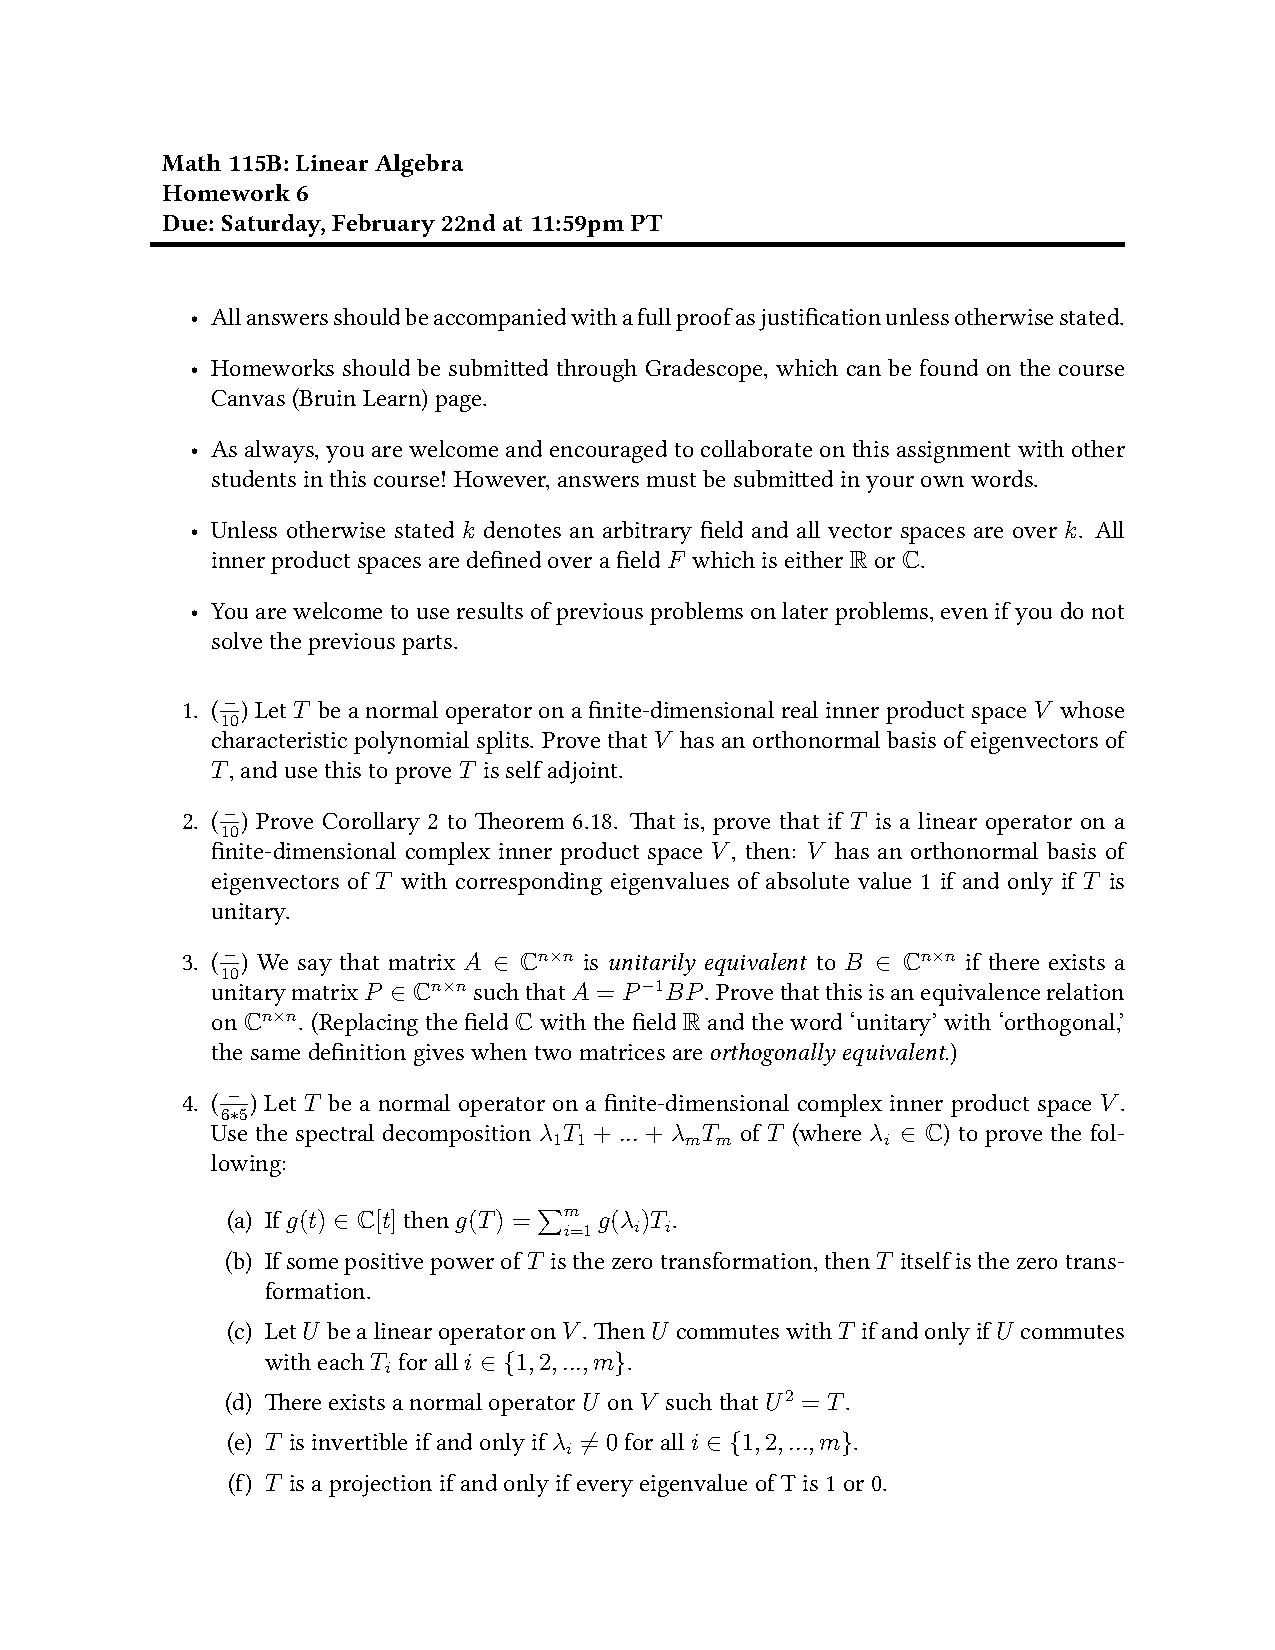
\includepdf[pages=-]{assignment.pdf}

\end{document}
